\begin{figure*}[!p]
  \centering
  \begin{subfigure}[b]{0.8\textwidth}
  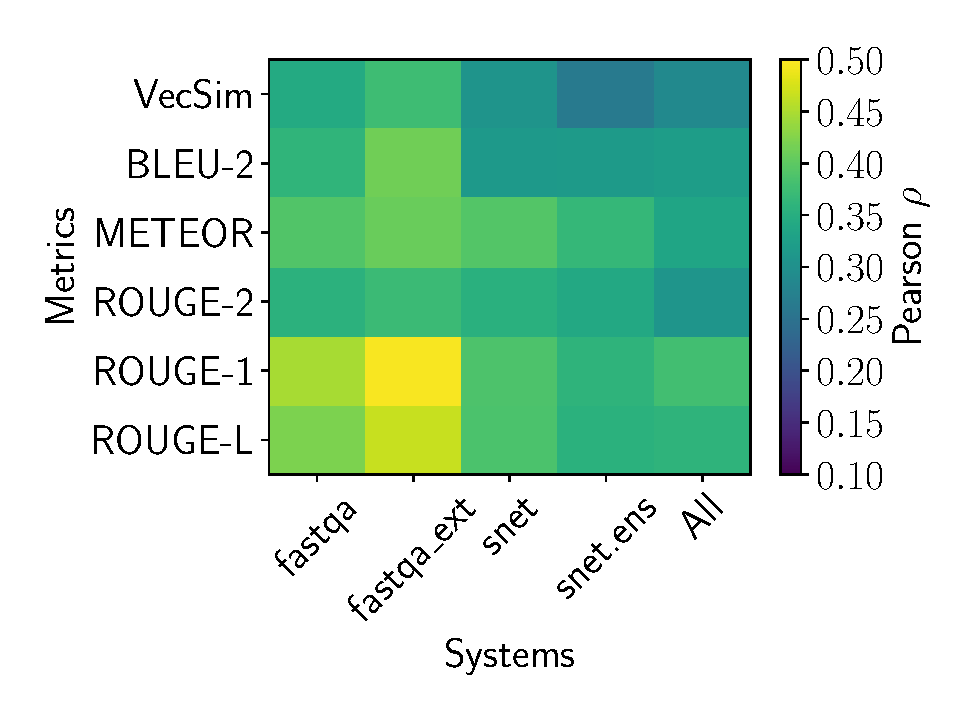
\includegraphics[width=\textwidth]{figures/msmarco_correlation}
  \caption{MS MARCO with the \texttt{AnyCorrect} prompt}
  \end{subfigure}

  \begin{subfigure}[b]{0.8\textwidth}
  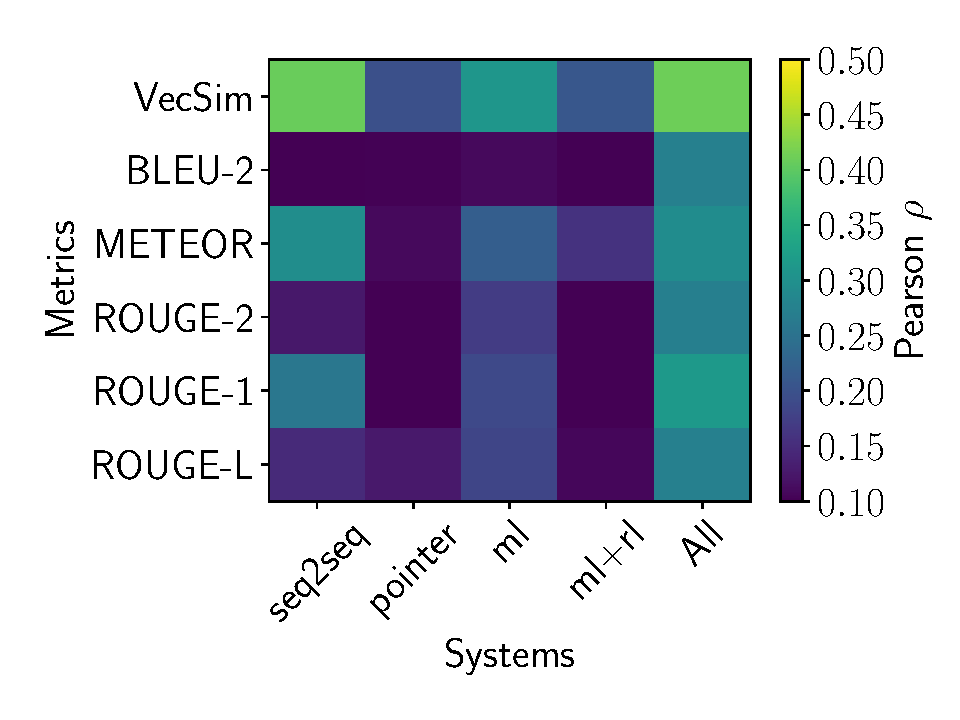
\includegraphics[width=\textwidth]{figures/lqual_correlation}
  \caption{CNN/Daily Mail with the \texttt{Edit} prompt}
  \end{subfigure}

  \caption[Correlations of different automatic metrics on the MS MARCO and CNN/Daily Mail tasks.]
{\label{fig:price:correlation} Correlations of different automatic metrics on the MS MARCO and CNN/Daily Mail tasks.
  Certain systems are more correlated with certain automatic metrics than others, but overall the correlation is low to moderate for most systems and metrics.
  }
\end{figure*}


\section{\label{sec:price:evaluation}Experimental results}

We are now ready to evaluate the performance of our control variates estimator proposed in \refsec{price:method} using the datasets presented in \refsec{price:tasks}.
Recall that our primary quantity of interest is \textit{data efficiency}, the ratio of the number of human judgments required to estimate the overall human evaluation score for the control variates estimator versus the sample mean.
We'll briefly review the automatic metrics used in our evaluation before analyzing the results.

%\begin{figure}[t]
%  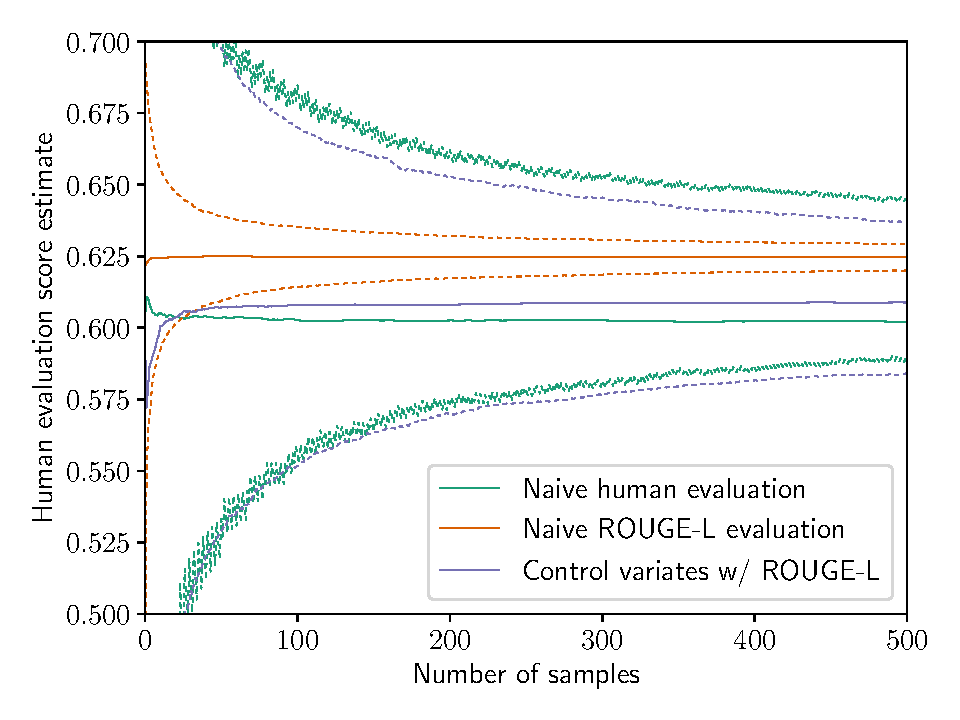
\includegraphics[width=\columnwidth]{figures/msmarco_full_trajectory}
%  \caption{\label{fig:bias-trajectory} A comparison of the human score estimates made by (a) naively sampling humans, (b) scaling and shifting the best automatic metric (ROUGE-L) and (c) incorporating the automatic metric into the control variates estimator proposed in this paper.
%  While (c) does not significantly reduce variance in its estimates, it is still an unbiased estimation of the human evaluation score, unlike (b).
%  The low confidence interval for the ROUGE-L scores are because they do not observe any annotator noise.
%  \ac{The curves are not exactly aligned because of a minor error in data for this plots. It will be fixed.}
%  }
%\end{figure}

% Evaluation
\paragraph{Automatic metrics.}
We consider the following frequently used automatic word-overlap based metrics in our work:
\textbf{BLEU}~\citep{papineni02bleu}, \textbf{ROUGE}~\citep{lin2004rouge} and \textbf{METEOR}~\citep{lavie2009meteor}.
Following \citet{novikova2017why} and \citet{liu2016evaluate}, we also compared a vector-based sentence-similarity using \texttt{sent2vec}~\citep{pagliardini2017unsupervised} to compare sentences (\textbf{VecSim}).
\reffig{price:correlation} shows how each of these metrics is correlated with human judgment for the systems being evaluated.
Unsurprisingly, the correlation varies considerably across systems, with token-based metrics correlating more strongly for systems that are more extractive in nature (\texttt{fastqa} and \texttt{fastqa\_ext}).

%\reffig{bias-trajectory} shows a trajectory estimates for human evaluation scores using the baseline of naive human evaluation versus those with the proposed control variates method.\footnote{%
%  All confidence intervals reported here are measured using 5,000 bootstrap samples generated by picking uniformly from the examples from the system output and then uniformly from the human annotations on that example.
%  }
%We also plot the estimate produced using an automatic metric, namely ROUGE-L after being scaled and shifted to match human evaluation scores at the system-level.
%Here, we see that while the control variates approach does not significantly reduce variance in estimates, it remains unbiased when using the model, unlike using the automatic metric.

%\begin{figure*}[t]
%  \centering
%  \begin{subfigure}[b]{0.45\textwidth}
%    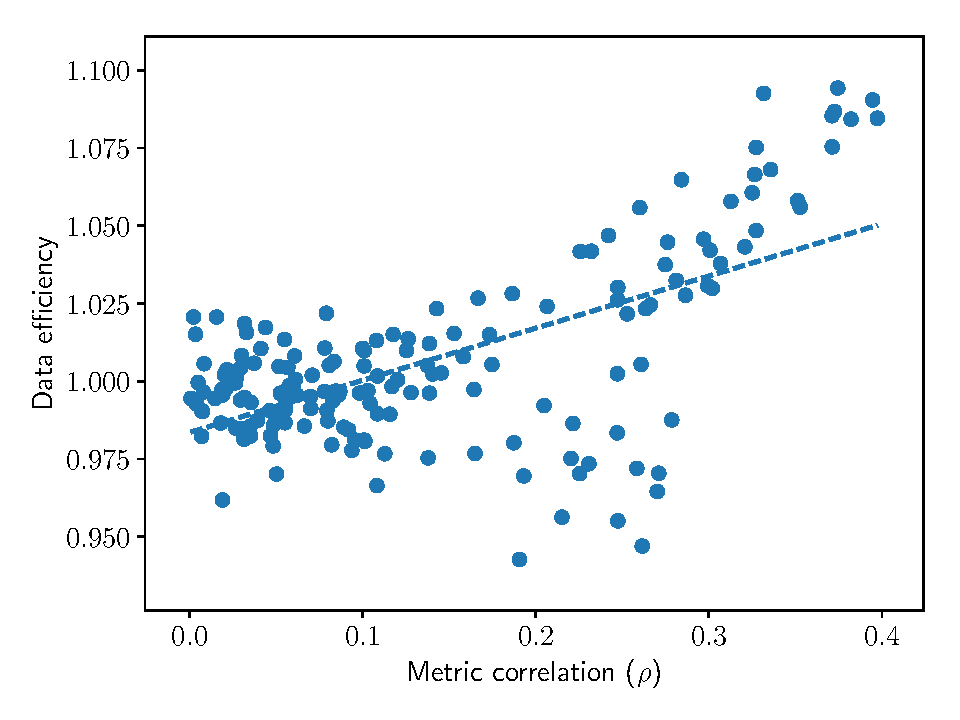
\includegraphics[width=\textwidth]{figures/de_vs_rho}
%  \end{subfigure} \hfill
%  \begin{subfigure}[b]{0.45\textwidth}
%    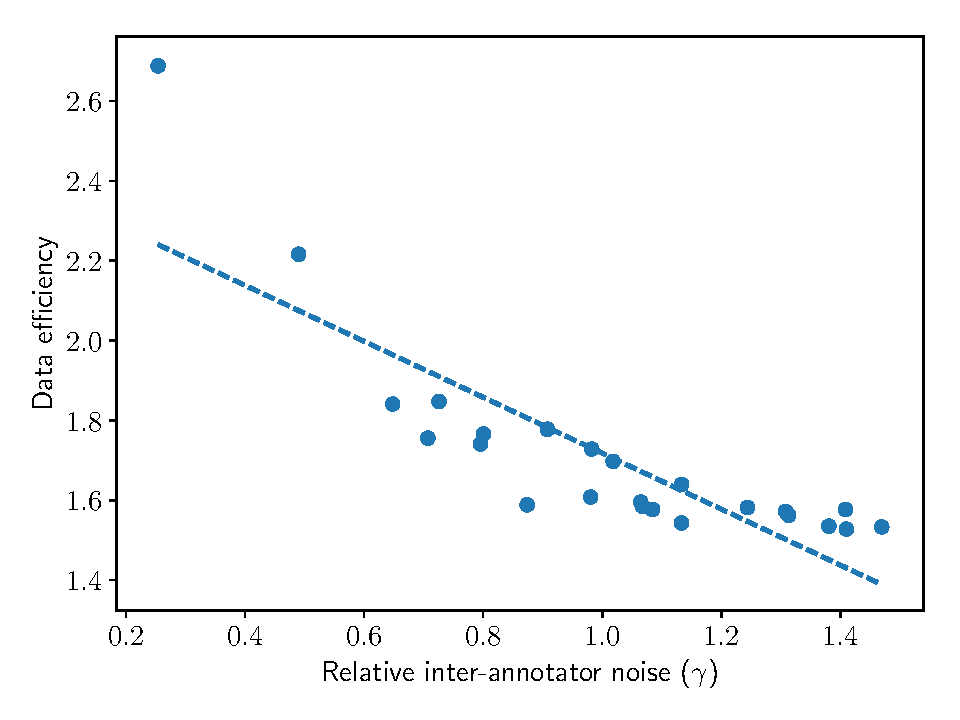
\includegraphics[width=\textwidth]{figures/de_vs_gamma}
%  \end{subfigure}
%  \caption{\label{fig:data-efficiency} A comparison of data efficiency possible across different systems and metrics. \ac{This figure seems like not very important so prefer ignoring.}}
%\end{figure*}

\begin{figure*}[!p]
  \centering
  \begin{subfigure}[t]{0.45\textwidth}
  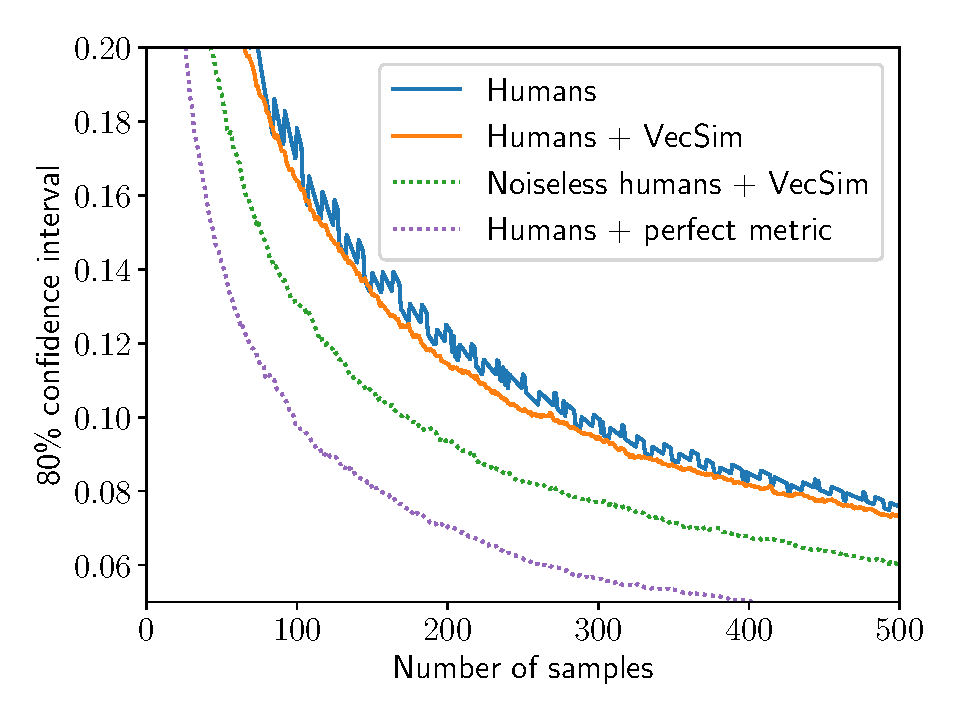
\includegraphics[width=\textwidth]{figures/lqual_trajectory_foil}
    \caption{\label{fig:price:trajectory-a}\texttt{seq2seq} on CNN/Daily Mail using the \texttt{Overall}}
  \end{subfigure} 
  \hfill
  \begin{subfigure}[t]{0.45\textwidth}
  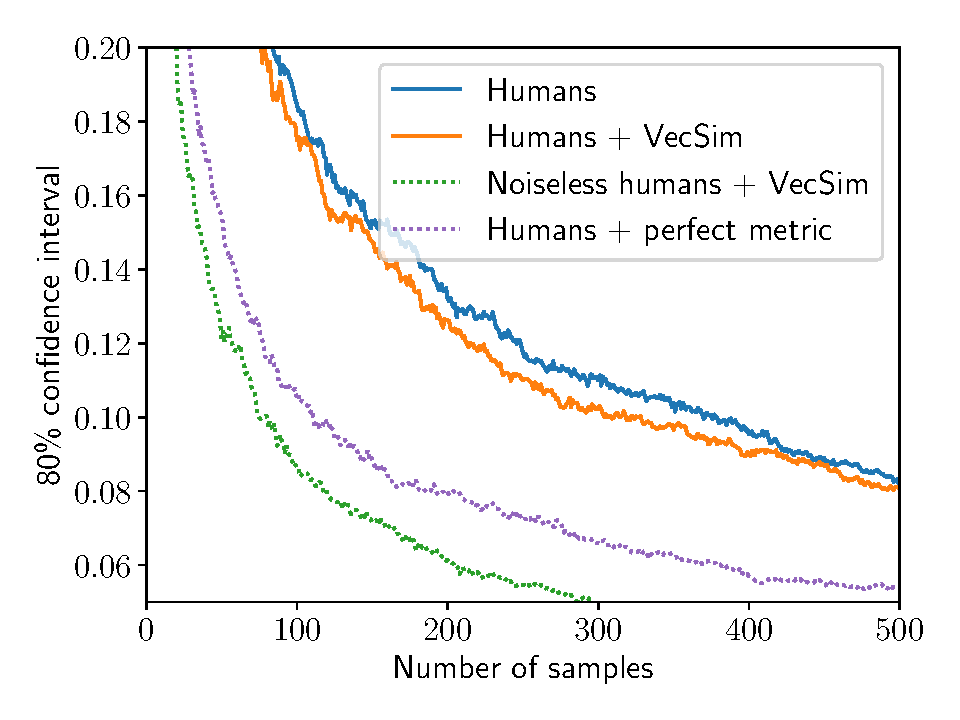
\includegraphics[width=\textwidth]{figures/lqual_trajectory}
  \caption{\label{fig:price:trajectory-b}\texttt{seq2seq} on CNN/Daily Mail using \texttt{Edit} }
  \end{subfigure}

  \begin{subfigure}[b]{0.6\textwidth}
  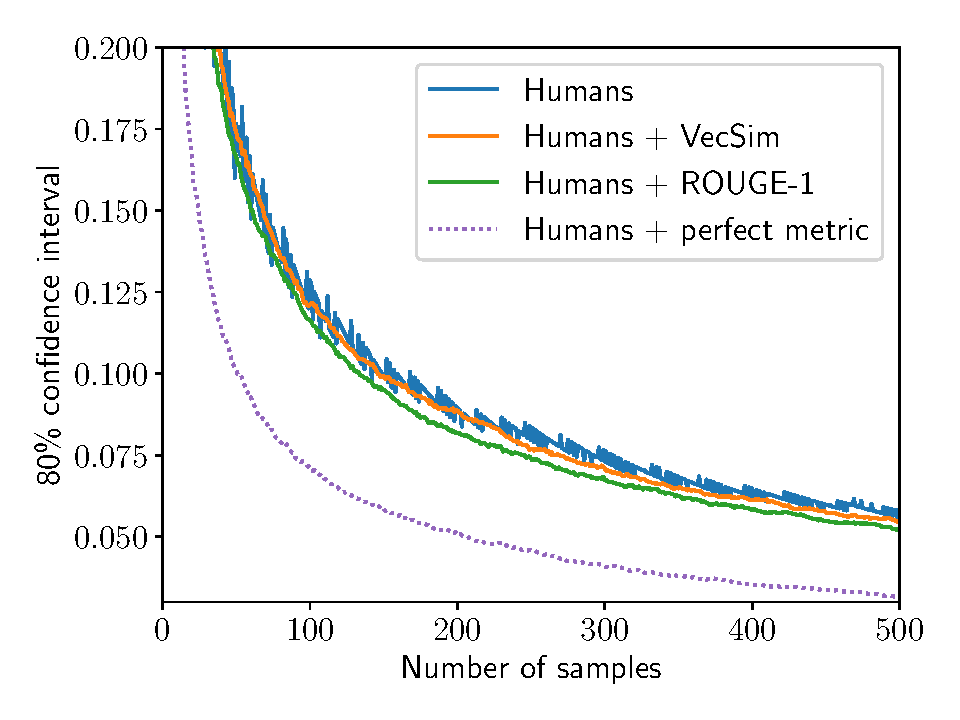
\includegraphics[width=\textwidth]{figures/msmarco_trajectory}
  \caption{\label{fig:price:trajectory-c}\texttt{fastqa\_ext} on MS MARCO using \texttt{AnyCorrect}}
  \end{subfigure}

  \caption[Confidence intervals as a function of the number of human judgments used when evaluating systems]{\label{fig:price:trajectory} 80\% bootstrap confidence interval length as a function of the number of human judgments used when evaluating the indicated systems on their respective datasets and prompts.
  (a) We see a modest reduction in variance (and hence cost) relative to human evaluation by using the VecSim automatic metric with the proposed control variates estimator to estimate \texttt{Overall} scores on the CNN/Daily Mail task; the data efficiency (DE) is $1.06$.
  (b) By improving the evaluation prompt to use \texttt{Edit}s instead, it is possible to further reduce variance relative to humans (DE is $1.15$).
  (c) Another way to reduce variance relative to humans is to improve the automatic metric evaluation; here using ROUGE-1 instead of VecSim improves the DE from $1.03$ to $1.16$.
  }
\end{figure*}

\paragraph{Results.}

In \refsec{price:method} we proved that the control variates estimator is not only unbiased but also has the least variance among other unbiased estimators.
\reffig{price:trajectory} plots the width of the 80\% confidence interval, estimated using bootstrap, measured as a function of the number of samples collected for different tasks and prompts.
As expected, the control variates estimator reduces the width of the confidence interval. 
We measure data efficiency by the averaging of the ratio of squared confidence intervals between the human baseline and control variates estimates.
We observe that the data efficiency depends on the task, prompt and system, ranging from about 1.08 (a 7\% cost reduction) to 1.15 (a 13\% cost reduction) using current automatic metrics.

As we showed in \refsec{price:method}, further gains are fundamentally limited by the quality of the evaluation prompts and automatic metrics.
\reffig{price:trajectory-a} and~\ref{fig:price:trajectory-b} show how improving the quality of the evaluation prompt from a Likert-scale prompt for quality (\texttt{Overall}) to using post-editing (\texttt{Edit}) noticeably decreases variance and hence allows better automatic metrics to increase data efficiency.
Likewise, \reffig{price:trajectory-c} shows how using a better automatic metric (ROUGE-L instead of VecSim) also reduces variance.

%Note that even we were used ``a perfect metric'', i.e.\ one that had a correlation $\rho = 1$, we must collect at least a few human annotations to find out if the metric is indeed correct. \stm{I covered this case in the method section. Cut?}
%As a result, we might expect that annotator noise will still limit the data efficiency when using a perfect metric.
\reffig{price:trajectory} also shows the conjectured confidence intervals if we were able to eliminate noise in human judgments (noiseless humans) or have a automatic metric that correlated perfectly with average human judgment (perfect metric).
In particular, we use the mean of all (2--3) humans on each $z$ for the perfect $g(z)$ and use the mean of all humans on each $z$ for the ``noiseless'' $Y(z)$.
% AC: We want to say that the conjectured confidence intervals are an over-estimate.
%  We note that using the mean of the human responses for the perfect $g(z)$ introduces some correlation with human responses
%These probably yield optimistic \pl{maybe just remove this sentence, because we're already being optimistic; this is additional optimism, which might be confusing} data efficiencies because we don't have access to the true mean $f(z)$; further, the estimated perfect $g(z)$ we use is correlated with human judgments and hence ``corrects'' for their variance.

In both cases, we are able to significantly increase data efficiency (i.e.\ decrease estimator variance).
%but the data efficiency is capped based on the automatic metrics' correlation or the annotator noise respectively.
With zero annotator variance and using existing automatic metrics,
the data efficiency ranges from 1.42 to 1.69. With automatic metrics with perfect correlation and current variance of human judgments,
it ranges from 2.38 to 7.25.
%as shown in \reffig{data-efficiency}.
Thus, we conclude that it is important not only to improve our automatic metrics but also the evaluation prompts we use during human evaluation. 
